\subsection{Secondary Energy Source}
Secondary Energy Sources, or commonly known as peaking units, are an essential part of the energy grid. These systems provide "on-demand" energy during moments when the electrical demand is larger than what the rest of the grid can accomodate. A common feature of 

\subsubsection{Natural Gas Fired Turbine}

Recently, natural gas-fired turbines have found widespread use because of their higher efficiencies, lower capital costs, shorter installation times, abundance of natural gas supplies, lower greenhouse gas emissions compared to other energy sources; and fast start-up capability, which enables them to be used as peaking units that respond to peak demands \cite{GasTurbine2008}, \cite{GasTurbine2013}. Due to their special characteristics, natural gas fired turbines are installed in numerous places around the world and have become an important source for power generation. This section is dedicated to detailed process and control designs of the GTPP, whose primary role is to cover rapid dynamics in grid demand that cannot be met by the remainder of the N-R HES. Simulation results involving several case studies are also provided. Full system details are available in OSTI \cite{2016HTSE}.

The natural gas turbine, Figure \ref{Top View Gas Turbine}, is designed with parameters embedded in each individual component. The top level variables can be edited directly within the GTTP\textunderscore PowerCtrl system. This component is where things such as pressure ratios, flow rates, mechanical efficiencies, and shaft inertia can be modified. The natural gas turbine is designed with a nominal electrical power generation capacity of 35MWe but has a specially designed capacityScaler variable that allows the user to scale the system to between 17 and 70MWe for a singular load. If more are desired then the deployment of several natural gas fired turbines would be required. 

\begin{figure}[hbtp]
\centering
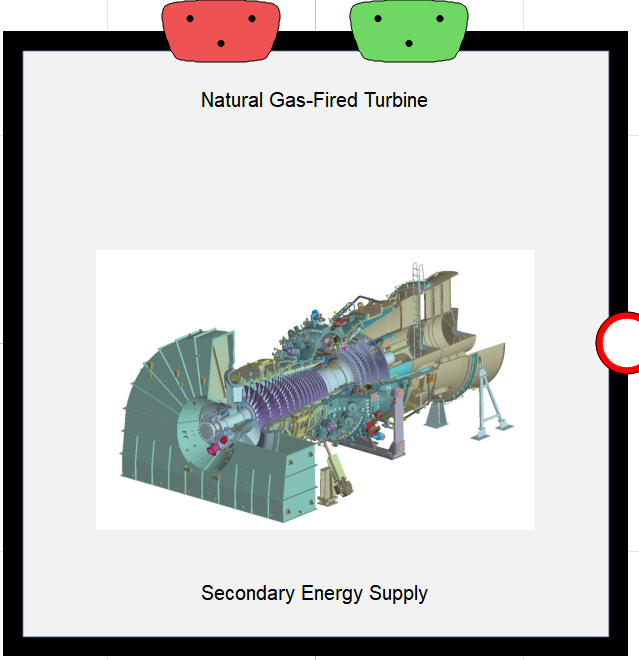
\includegraphics[scale=0.4]{pics/GasTurbine.png}
\caption{Top Level Depiction of the Natural Gas Fired Turbine in the NHES package}
\label{Top View Gas Turbine}
\end{figure}

\subsubsection{Hydrogen Turbine}
With the increase in hydrogen production technologies comes on the other end hydrogen burning technologies. To accommodate a hydrogen burning technology the HYBRID repository has been outfitted with a retrofit natural gas burner that is capable of handling pure hydrogen. 

The hydrogen turbine, Figure \ref{Top View Hydrogen Turbine}, is designed with parameters embedded in each individual component. The top level variables can be edited directly within the Hydrogen\textunderscore PowerCtrl system. This component is where things such as pressure ratios, flow rates, mechanical efficiencies, and shaft inertia can be modified. The hydrogen turbine is designed with a nominal electrical power generation capacity of 35MWe but has a specially designed capacityScaler variable that allows the user to scale the system to between 17 and 70MWe for a singular load. If more are desired then the deployment of several hydrogen turbines would be required. 


\begin{figure}[hbtp]
\centering
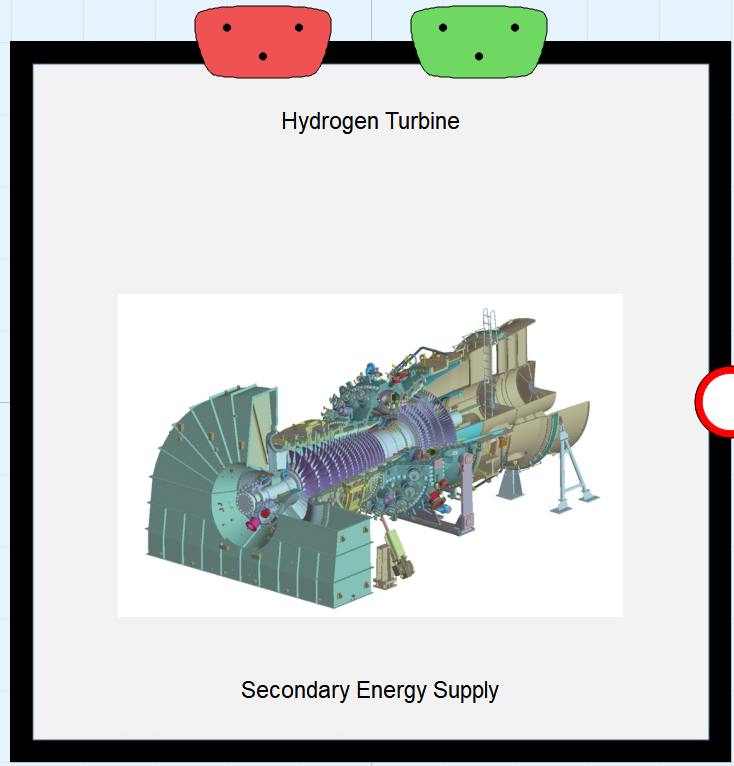
\includegraphics[scale=0.4]{pics/Hydrogen_Turbine.png}
\caption{Top Level Depiction of the Hydrogen Turbine in the NHES package}
\label{Top View Hydrogen Turbine}
\end{figure}
%\subsection{Cloning the Hybrid Repository}
\label{sec:clone raven}

The first step in installing the package is to clone the HYBRID repository. To do this, use
\begin{lstlisting}[language=bash]
git clone https://github.com/idaholab/HYBRID.git
\end{lstlisting}
This will download the repository into a folder called 'hybrid'. To go inside the folder, use
\begin{lstlisting}[language=bash]
cd hybrid
\end{lstlisting}


\subsubsection{Install RAVEN and its plugins as a sub-module}

The next step is to download and install RAVEN and the submodule (e.g. TEAL, HERON) plugins as a sub-module of the HYBRID repository. 

A submodule allows you to keep another Git repository in a subdirectory of your repository. The other repository has its own history, which does not interfere with the history of the current repository. This can be used to have external dependencies such as third party libraries for example.

In order to get RAVEN do the following in the hybrid folder

\begin{lstlisting}[language=bash]
git checkout devel
\end{lstlisting}

Update the Branch

\begin{lstlisting}[language=bash]
git pull
\end{lstlisting}

to add RAVEN as a submodule
\begin{lstlisting}[language=bash]
git submodule update --init --recursive
\end{lstlisting}

\textbf{Install and Compile RAVEN. }
Once you have downloaded RAVEN as a sub-module, you have to install it. go to the \href{https://github.com/idaholab/raven/wiki/intallationMain}{RAVEN Wiki} for information about how to install it. Run all the tests outlined in the RAVEN wiki. 

\subsubsection{Inform the Framework Paths}

In order to set up the hybrid repository, you must inform the framework about the location of the Dymola python interface. For doing so, navigate to the hybrid directory:

to add RAVEN as a submodule
\begin{lstlisting}[language=bash]
cd <path to your hybrid repository>/hybrid
\end{lstlisting}
Run the following command:
\begin{lstlisting}[language=bash]
./scripts/write_hybridrc.py -p DYMOLA_PATH
\end{lstlisting}

Where DYMOLAPATH is the path to the python interface egg folder in the DYMOLA installation locally. For example:
 
\begin{lstlisting}[language=bash]
./scripts/write_hybridrc.py -p 
	"/c/Program\ Files/Dymola\ 2020x/Modelica/Library/
	python_interface/dymola.egg"
\end{lstlisting}

